\documentclass{article}
\usepackage{tikz}
\usepackage{tikz-cd}
\usetikzlibrary{matrix,positioning,intersections}
\usepackage{amsmath}
\usepackage{amssymb}
\usepackage{mathtools}
\usepackage{booktabs}
\usepackage{algorithm2e}
\usepackage{algpseudocode}

\title{Weird Algorithms}
\author{Amy Wilder}

\setlength{\parskip}{10pt}
\SetAlgoLined{}
\SetKwComment{Comment}{/* }{ */}
\RestyleAlgo{ruled}
\DontPrintSemicolon{}

\begin{document}

\maketitle

\section{Compare All Sort}

The Compare All sorting algorithm is an alternative to Counting Sort which can be used with collections of integers of any value, or even non-integers with defined comparison operators.

The algorithm achieves this by comparing each element in the collection against every other element in the collection to determine the sorted index of each element.

To operate, the algorithm requires one of two buffers in addition to the original array, each of which would have the same number of elements as the original array.

The first of these, hereafter referred to as the ``Index Array'', will store the indices of each element in the original array sorted by associated value.
These are found by counting the number of elements in the original array whose values come before\footnote{
    The comparison may be strictly less than, or less than or equal to.
    This is dependent on the position in the original array of the element being inspected, relative to that of the element being sorted.
} that of the element at the corresponding position in the original array.

The second acts as a buffer for storing the unsorted values of the original array.
This is used to prevent the Index Array's values from becoming invalidated while shifting the original array's elements.
Whether the buffer is used to output the sorted array, or to store a copy of the unsorted array while overwriting the elements in the original, is up to implementation.

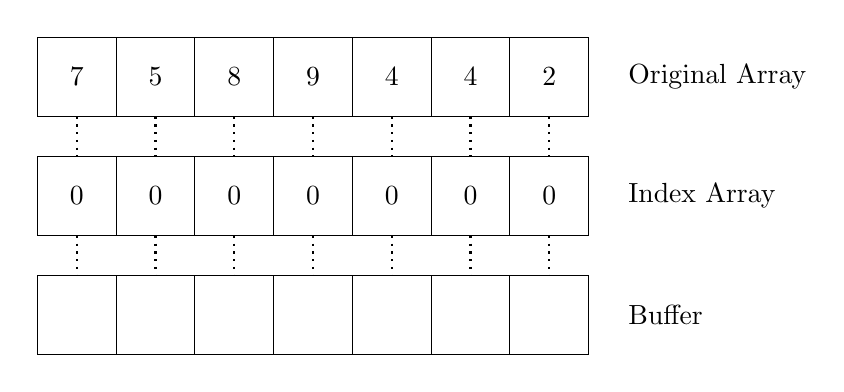
\begin{tikzpicture}
    \matrix (original array) [matrix of nodes, nodes in empty cells,
        nodes={draw, minimum size=1cm, anchor=center},
        column sep=-\pgflinewidth, row sep=-\pgflinewidth
    ]{
        7 & 5 & 8 & 9 & 4 & 4 & 2 \\
    };

    \node[right=0.25cm of original array.east] {Original Array};

    \matrix (index array) [matrix of nodes, nodes in empty cells,
        nodes={draw, minimum size=1cm, anchor=center},
        column sep=-\pgflinewidth, row sep=-\pgflinewidth,
        below=0.25cm of original array
    ]{
        0 & 0 & 0 & 0 & 0 & 0 & 0 \\
    };

    \node[right=0.25cm of index array.east] {Index Array};

    \matrix (buffer) [matrix of nodes, nodes in empty cells,
        nodes={draw, minimum size=1cm, anchor=center},
        column sep=-\pgflinewidth, row sep=-\pgflinewidth,
        below=0.25cm of index array
    ]{
        ~ & ~ & ~ & ~ & ~ & ~ & ~ \\
    };

    \node[right=0.25cm of buffer.east] {Buffer};

    \foreach \i in {1,...,7}{
        \draw[thick,dotted] (original array-1-\i.south) -- (index array-1-\i.north);
        \draw[thick,dotted] (index array-1-\i.south) -- (buffer-1-\i.north);
    }
\end{tikzpicture}

\begin{samepage}
To execute the algorithm, iterate over each index \( i \) and each other index \( j \) in the original array
\begin{itemize}
    \item Where \( j < i \), count the number of \( j \)-elements with values less than or equal to the value of the \( i \)-element.
    \item Where \( j = i \), do nothing.
    \item Where \( j > i \), count the number of \( j \)-elements with values strictly less than the value of the \( i \)-element.
\end{itemize}

\nopagebreak
That is to say:

\nopagebreak
\noindent
let \( A \) be the original array, \( I \) be the index array, and \( n \) be the length of \( A \). Then,

\[
    I_i =
    \sum_{j = 1}^{n}
    \begin{cases}
        A_j \le A_i & j < i \\
        \text{skip} & j = i \\
        A_j  <  A_i & j > i
    \end{cases}
\]

\nopagebreak
The accumulated result once all elements \( j \) have been inspected is assigned to the Index Array at the position corresponding with element \( i \).
\end{samepage}

\begin{samepage}
For example:

\nopagebreak
Start at element \( i = 1 \), whose value is 7, skipping \( j \) where \( j = i \):

\nopagebreak
4 values strictly less than 7 exist in the array: 5, 4, 4, and 2; so the value at position \( i = 1 \) of the Index Array is 4.

\nopagebreak
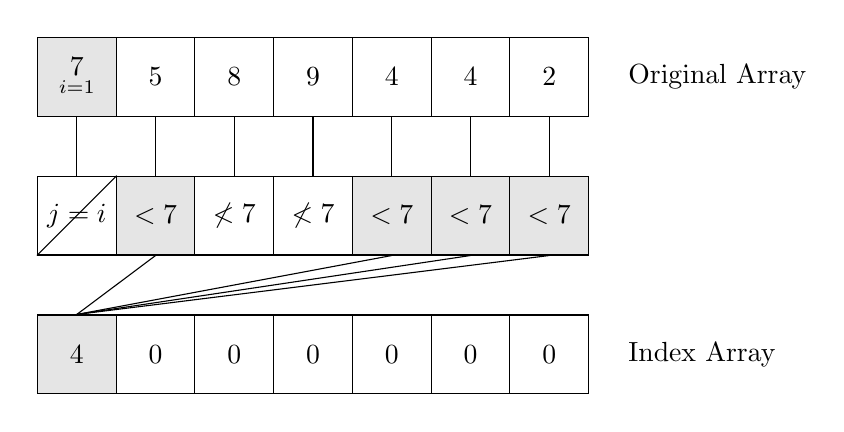
\begin{tikzpicture}
    \matrix (original array) [matrix of nodes, nodes in empty cells,
        nodes={draw, minimum size=1cm, anchor=center},
        column sep=-\pgflinewidth, row sep=-\pgflinewidth
    ]{
        |[fill=gray!20]| \( \underset{i = 1}{7} \) & 5 & 8 & 9 & 4 & 4 & 2 \\
    };
    \node[right=0.25cm of original array.east] {Original Array};

    \matrix (comparison array) [matrix of nodes, nodes in empty cells,
        nodes={draw, minimum size=1cm, anchor=center},
        column sep=-\pgflinewidth, row sep=-\pgflinewidth,
        below=0.5cm of original array
    ]{
        \( j = i \) &
        |[fill=gray!20]| \(< 7\) &
        \(\not< 7\) &
        \(\not< 7\) &
        |[fill=gray!20]| \(< 7\) &
        |[fill=gray!20]| \(< 7\) &
        |[fill=gray!20]| \(< 7\) \\
    };
    \draw (comparison array-1-1.south west) -- (comparison array-1-1.north east);

    \foreach \i in {1,...,7}
        \draw (original array-1-\i.south) -- (comparison array-1-\i.north);

    \matrix (index array) [matrix of nodes, nodes in empty cells,
        nodes={draw, minimum size=1cm, anchor=center},
        column sep=-\pgflinewidth, row sep=-\pgflinewidth,
        below=0.5cm of comparison array
    ]{
        |[fill=gray!20]| 4 & 0 & 0 & 0 & 0 & 0 & 0 \\
    };
    \node[right=0.25cm of index array.east] {Index Array};

    \foreach \i in {2,5,6,7}
        \draw (comparison array-1-\i.south) -- (index array-1-1.north);
\end{tikzpicture}

\nopagebreak
Because an array may contain duplicate values, elements of index \( j < i \) are inspected with \( A_j \le A_i \) instead of \( A_j < A_i \).
This allows duplicates to remain in their original order with respect to each other, while sorting the duplicates with respect to all other elements.
\end{samepage}

For an example of this, consider \( i = 5 \) and \( i = 6 \).

\begin{samepage}
First, \( i = 5 \):

\nopagebreak
The element \( i = 5 \) has a value of 4.
So only one value, 2, meets the criteria to be counted; making the value at position \( i = 5 \) of the Index Array 1.

\nopagebreak
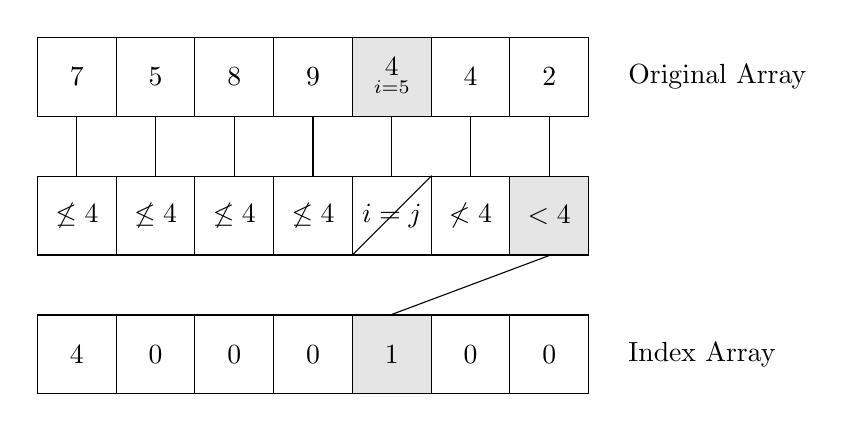
\begin{tikzpicture}
    \matrix (original array) [matrix of nodes, nodes in empty cells,
        nodes={draw, minimum size=1cm, anchor=center},
        column sep=-\pgflinewidth, row sep=-\pgflinewidth
    ]{
        7 & 5 & 8 & 9 & |[fill=gray!20]| \( \underset{i = 5}{4} \) & 4 & 2 \\
    };
    \node[right=0.25cm of original array.east] {Original Array};

    \matrix (comparison array) [matrix of nodes, nodes in empty cells,
        nodes={draw, minimum size=1cm, anchor=center},
        column sep=-\pgflinewidth, row sep=-\pgflinewidth,
        below=0.5cm of original array
    ]{
        \(\not\le 4\) &
        \(\not\le 4\) &
        \(\not\le 4\) &
        \(\not\le 4\) &
        \( i = j \) &
        \(\not< 4\) &
        |[fill=gray!20]| \(< 4\) \\
    };
    \draw (comparison array-1-5.south west) -- (comparison array-1-5.north east);

    \foreach \i in {1,...,7}
        \draw (original array-1-\i.south) -- (comparison array-1-\i.north);

    \matrix (index array) [matrix of nodes, nodes in empty cells,
        nodes={draw, minimum size=1cm, anchor=center},
        column sep=-\pgflinewidth, row sep=-\pgflinewidth,
        below=0.5cm of comparison array
    ]{
        4 & 0 & 0 & 0 & |[fill=gray!20]| 1 & 0 & 0 \\
    };
    \node[right=0.25cm of index array.east] {Index Array};

    \draw (comparison array-1-7.south) -- (index array-1-5.north);
\end{tikzpicture}
\end{samepage}

\begin{samepage}
Now, \( i = 6 \):

\nopagebreak
The element \( i = 6 \) also has a value of 4.
So two values, 4 and 2, meet the criteria to be counted; making the value at position \( i = 6 \) of the Index Array 2.

\nopagebreak
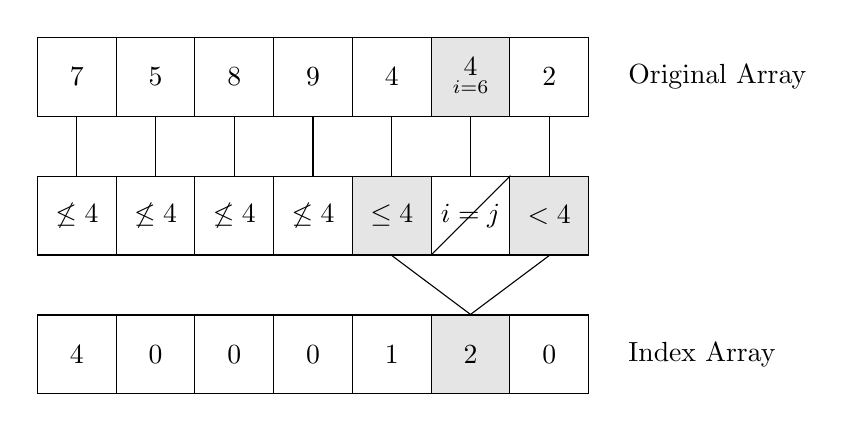
\begin{tikzpicture}
    \matrix (original array) [matrix of nodes, nodes in empty cells,
        nodes={draw, minimum size=1cm, anchor=center},
        column sep=-\pgflinewidth, row sep=-\pgflinewidth
    ]{
        7 & 5 & 8 & 9 & 4 & |[fill=gray!20]| \( \underset{i = 6}{4} \) & 2 \\
    };
    \node[right=0.25cm of original array.east] {Original Array};

    \matrix (comparison array) [matrix of nodes, nodes in empty cells,
        nodes={draw, minimum size=1cm, anchor=center},
        column sep=-\pgflinewidth, row sep=-\pgflinewidth,
        below=0.5cm of original array
    ]{
        \(\not\le 4\) &
        \(\not\le 4\) &
        \(\not\le 4\) &
        \(\not\le 4\) &
        |[fill=gray!20]| \(\le 4\) &
        \( i = j \) &
        |[fill=gray!20]| \(< 4\) \\
    };
    \draw (comparison array-1-6.south west) -- (comparison array-1-6.north east);

    \foreach \i in {1,...,7}
        \draw (original array-1-\i.south) -- (comparison array-1-\i.north);

    \matrix (index array) [matrix of nodes, nodes in empty cells,
        nodes={draw, minimum size=1cm, anchor=center},
        column sep=-\pgflinewidth, row sep=-\pgflinewidth,
        below=0.5cm of comparison array
    ]{
        4 & 0 & 0 & 0 & 1 & |[fill=gray!20]| 2 & 0 \\
    };
    \node[right=0.25cm of index array.east] {Index Array};

    \foreach \i in {5,7}
        \draw (comparison array-1-\i.south) -- (index array-1-6.north);
\end{tikzpicture}
\end{samepage}

\begin{samepage}
By applying this method to each element \( i \) of the original array, we get the following result:

\nopagebreak
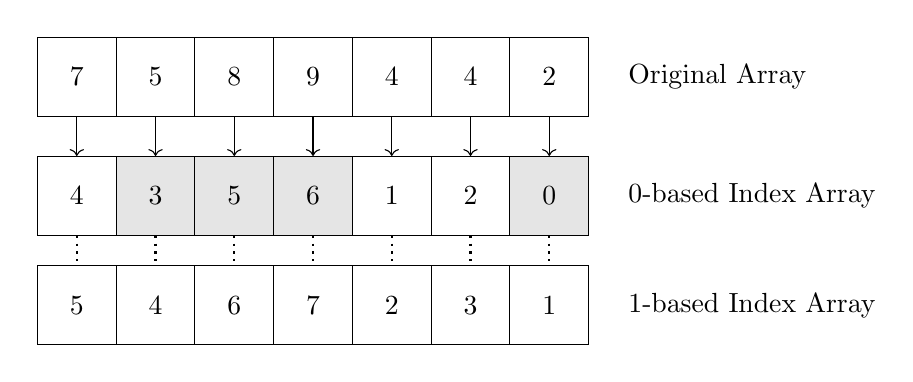
\begin{tikzpicture}
    \matrix (original array) [matrix of nodes, nodes in empty cells,
        nodes={draw, minimum size=1cm, anchor=center},
        column sep=-\pgflinewidth, row sep=-\pgflinewidth
    ]{
        7 & 5 & 8 & 9 & 4 & 4 & 2 \\
    };

    \node[right=0.25cm of original array.east] {Original Array};

    \matrix (index array 0) [matrix of nodes, nodes in empty cells,
        nodes={draw, minimum size=1cm, anchor=center},
        column sep=-\pgflinewidth, row sep=-\pgflinewidth,
        below=0.25cm of original array
    ]{
        4 & |[fill=gray!20]| 3 & |[fill=gray!20]| 5 & |[fill=gray!20]| 6 & 1 & 2 & |[fill=gray!20]| 0 \\
    };

    \node[right=0.25cm of index array 0.east] {0-based Index Array};

    \foreach \i in {1,...,7}
        \draw[->] (original array-1-\i.south) -- (index array 0-1-\i.north);

    \matrix (index array 1) [matrix of nodes, nodes in empty cells,
        nodes={draw, minimum size=1cm, anchor=center},
        column sep=-\pgflinewidth, row sep=-\pgflinewidth,
        below=0.125cm of index array 0
    ]{
        5 & 4 & 6 & 7 & 2 & 3 & 1 \\
    };

    \node[right=0.25cm of index array 1.east] {1-based Index Array};

    \foreach \i in {1,...,7}
        \draw[thick,dotted] (index array 0-1-\i.south) -- (index array 1-1-\i.north);
\end{tikzpicture}
\end{samepage}

\begin{samepage}
Finally, the elements of the original array are ordered such that each one's new index is that of the value in the Index Array corresponding with its current index. So,
\[ A'_i = A_{I_i} \]

\nopagebreak
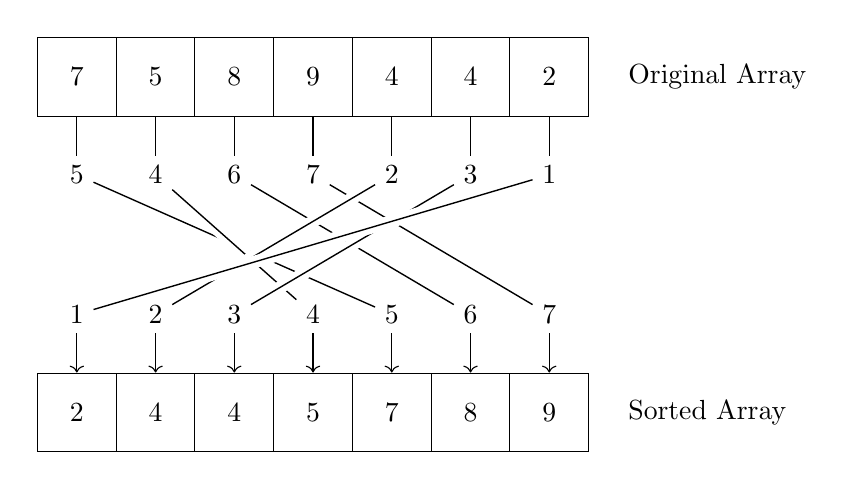
\begin{tikzpicture}
    \tikzset{
      link/.style = { white, double = black, line width = 2pt, double distance = 0.5pt },
    }
    \matrix (original array) [matrix of nodes, nodes in empty cells,
        nodes={draw, minimum size=1cm, anchor=center},
        column sep=-\pgflinewidth, row sep=-\pgflinewidth
    ]{
        7 & 5 & 8 & 9 & 4 & 4 & 2 \\
    };

    \node[right=0.25cm of original array.east] {Original Array};

    \foreach \n [count = \i] in {5,4,6,7,2,3,1}
        \node[below=0.5cm of original array-1-\i.south] (index array-\i) {\n};

    \matrix (sorted array) [matrix of nodes, nodes in empty cells,
        nodes={draw, minimum size=1cm, anchor=center},
        column sep=-\pgflinewidth, row sep=-\pgflinewidth,
        below=3cm of original array
    ]{
        2 & 4 & 4 & 5 & 7 & 8 & 9 \\
    };

    \node[right=0.25cm of sorted array.east] {Sorted Array};

    \foreach \i in {1,...,7}
        \node[above=0.5cm of sorted array-1-\i.north] (sorted index-\i) {\i};

    \foreach \n [count = \i] in {5,4,6,7,2,3,1} {
        \draw (original array-1-\i.south) -- (index array-\i);
        \draw[link] (index array-\i) -- (sorted index-\n);
        \draw[->] (sorted index-\n) -- (sorted array-1-\n.north);
    }
\end{tikzpicture}
\end{samepage}

\begin{samepage}
The clear drawbacks of this algorithm are that it has a time complexity of \(\mathcal{O}(n^2)\) (every element must be compared with every other element)
and a space complexity of \(\mathcal{O}(n)\) (either a buffer of the original collection's elements, or a collection of its sorted indices).

\nopagebreak
Of note however, the algorithm's time complexity is consistent regardless of the original array's order prior to sorting.
\(\mathcal{O}(n^2)\) is not only the average case, but also the worst \emph{and} best case.

\nopagebreak
\begin{center}
    \begin{tabular}{ cccc }
        \multicolumn{3}{ c }{Time Complexity} & Space Complexity \\
        \toprule
        Best Case & Average Case & Worst Case & Worst Case \\
        \midrule
        \(\mathcal{O}(n^2)\) & \(\mathcal{O}(n^2)\) & \(\mathcal{O}(n^2)\) & \(\mathcal{O}(n)\) \\
        \bottomrule
    \end{tabular}
\end{center}
\end{samepage}

\clearpage

\begin{samepage}
The following is an example of a Compare All Sort algorithm optimized for focus on iterators instead of obtaining a sorted copy of the original array.

\nopagebreak
This version has time complexity \(\mathcal{O}(n^2)\) in all cases.
If only iterating, it has space complexity \(\mathcal{O}(n)\).
If this version is used to obtain a sorted copy of the original array, it will have space complexity \(\mathcal{O}(2n)\).
For this reason, it is recommended to use algorithm~\ref{alg:compare all buffered} if a sorted copy is desired.

\nopagebreak
\begin{algorithm}[H]
    \caption{Compare All Sort --- Indexed}\label{alg:compare all indexed}
    \KwData{\(A\)}
    \KwResult{\(I\)}
    \(S \gets \) start-iterator of \(A\) \;
    \(E \gets \) end-iterator of \(A\) \;
    \(I \gets \) collection of \(A\)-iterators \;
    \ForEach{\(i \gets S\) \KwTo{\(E\)}} {
        \(I_i \gets S\) \;
        \BlankLine{}
        \ForEach{\(j \gets S\) \KwTo{\(i\)}} {
            \If{\(A_j \le A_i\)} {
                \(I_i \gets I_i + 1\) \;
            }
        }
        \BlankLine{}
        \ForEach{\(j \gets i + 1\) \KwTo{\(E\)}} {
            \If{\(A_j < A_i\)} {
                \(I_i \gets I_i + 1\) \;
            }
        }
        \BlankLine{}
        \Comment{Final sorted index of \(A_i\) is already known here.}
    }
    \BlankLine{}
    \Comment{\(I\) now holds each of \(A\)'s iterators sorted by value.}
\end{algorithm}
\end{samepage}

\clearpage

\begin{samepage}
The following is an example of a Compare All Sort algorithm optimized for obtaining a sorted copy of the original array without storing a collection of iterators.

\nopagebreak
This version has identical time complexity, but space complexity \(\mathcal{O}(n)\).

\nopagebreak
\begin{algorithm}[H]
    \caption{Compare All Sort --- Buffered}\label{alg:compare all buffered}
    \KwData{\(A\)}
    \KwResult{\(B\)}
    \(S \gets \) start-iterator of \(A\) \;
    \(E \gets \) end-iterator of \(A\) \;
    \(B \gets \) collection of (\(E-S\)) \(A\)-elements \;
    \ForEach{\(i \gets S\) \KwTo{\(E\)}} {
        \(n \gets S\) \;
        \BlankLine{}
        \ForEach{\(j \gets S\) \KwTo{\(i\)}} {
            \If{\(A_j \le A_i\)} {
                \(n \gets n + 1\) \;
            }
        }
        \BlankLine{}
        \ForEach{\(j \gets i + 1\) \KwTo{\(E\)}} {
            \If{\(A_j < A_i\)} {
                \(n \gets n + 1\) \;
            }
        }
        \BlankLine{}
        \(B_i \gets A_{n}\) \;
    }
\end{algorithm}
\end{samepage}

\end{document}
